%
% Ejemplos paquete Tikz.tex -- a document for writing notes with GEM.
%
% Copyright © 2017 Luis Felipe Villavicencio<lvillavicenciol@uni.pe>
%
% This program is free software: you can redistribute it and/or modify
% it under the terms of the GNU General Public License as published by
% the Free Software Foundation, either version 3 of the License, or
% (at your option) any later version.
%
% This program is distributed in the hope that it will be useful,
% but WITHOUT ANY WARRANTY; without even the implied warranty of
% MERCHANTABILITY or FITNESS FOR A PARTICULAR PURPOSE.  See the
% GNU General Public License for more details.
%
% You should have received a copy of the GNU General Public License
%s along with this program.  If not, see <http://www.gnu.org/licenses/>.
%
\documentclass{article}
\usepackage{tikz}
%\usepackage[spanish]{babel}
\usepackage[utf8]{inputenc}
\usetikzlibrary{babel} % Si van a usar Spanish como idioma
\usetikzlibrary[patterns]

\begin{document}
	
\begin{tikzpicture}
	\draw (0,0) -- (5,0);
	\draw[color=blue] (0,-1) -- (5,-1);
	\draw[color=blue,<->] (0,-2) -- (5,-2);
	\draw[color=blue,|<->|] (0,-3) -- (5,-3);
\end{tikzpicture}
	
\vspace{2cm}

Podemos también unir varios caminos.
\vspace{1cm} \newline
	
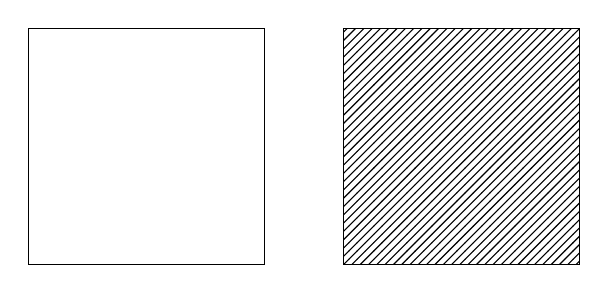
\begin{tikzpicture}
	\draw (0,0) -- (3,0) -- (3,3) -- (0,3) -- (0,0);
	\draw[fill=black,pattern=north east lines,pattern color=black] (4,0) -- (7,0) -- (7,3) -- (4,3) -- cycle;
\end{tikzpicture}
\vspace{1cm} \newline


\begin{tikzpicture}
\draw[ultra thick,fill=yellow,draw=orange] (0,0) -- (3,0) -- (3,3) -- (0,3) -- (0,0);
\draw[dashed] (4,0) -- (7,0) -- (7,3) -- (4,3) -- cycle;
\draw[dotted] (8,0) -- (11,0) -- (11,3) -- (8,3) -- cycle;
\end{tikzpicture}

\section{Dibujos}

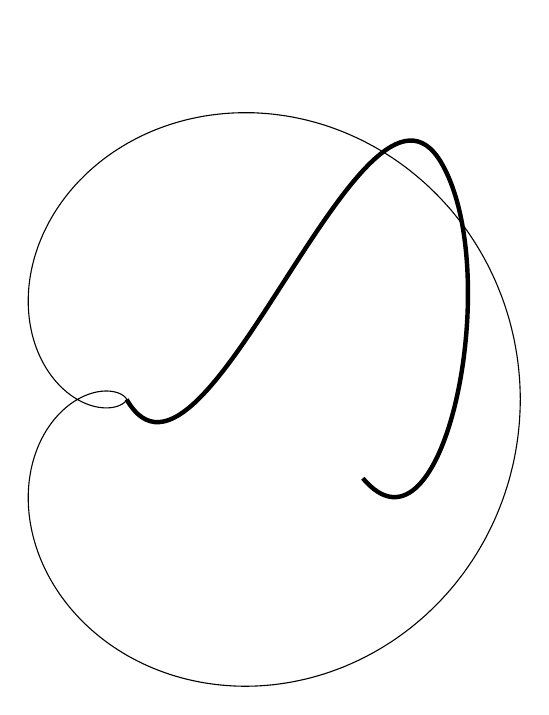
\begin{tikzpicture}
	\draw[ultra thick ] (0,0) to[in=120,out=-60]  (4,3) to[in=-50,out=-60] (3,-1) ;
	\draw[domain=0:540,scale=5,samples=500] plot (\x:{cos(\x/3)^3});		
\end{tikzpicture}
	
\newpage
	
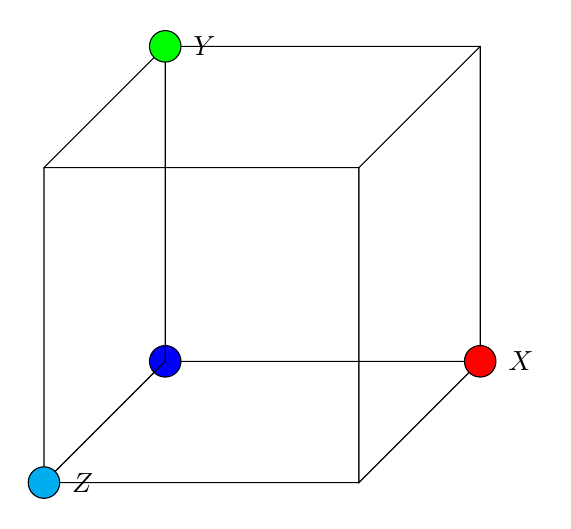
\begin{tikzpicture}
	\draw (0,0,0) -- (4,0,0) -- (4,4,0)--(0,4,0)--(0,4,4)--(4,4,4)--(4,0,4)--(4,0,0)--(0,0,0) --(0,0,4) -- (0,4,4);
	\draw[fill=blue](0,0,0) circle(0.2);
	\draw(4,4,0)--(4,4,4)--(4,0,4)--(0,0,4)--(0,0,0)--(0,4,0);
	
	\draw[fill=red](4,0,0) circle(0.2);
	\draw[fill=green](0,4,0) circle(0.2);
	\draw[fill=cyan](0,0,4) circle(0.2);
	\draw (4,0,0) node[right] {$~~X$};
	\draw (0,4,0) node[right] {$~~Y$};
	\draw (0,0,4) node[right] {$~~Z$};
\end{tikzpicture}

\end{document}